\section{Variance estimation with imputed data}\label{variance-estimation}
% 2.1 Data structure and notation
\subsection{Data structure and notation}\label{data-notation}
We observe independent and identically distributed data
\(O_1,\ldots,O_n\), where each \(O_i\) records the components that are
observed for subject \(i\) together with its missingness pattern.  We
write \(Z_i\) for the complete data of subject \(i\): the ideal data we
would wish to observe on every subject, comprising both the observed
and the missing components.  Throughout, \(P_n\) denotes the empirical
average, \(P_n f = n^{-1}\sum_{i=1}^n f_i\).
The parameter of interest is a finite-dimensional parameter
\(\beta\in\mathbb{R}^q\) defined through a complete-data estimating
function \(U(\cdot\,;\beta)\) as the unique solution of the population
estimating equation \(E\{U(Z;\beta_0)\}=0\).  This formulation is
general: \(\beta\) need not be a regression coefficient, but can be any
parameter admitting an unbiased complete-data estimating function.  We
call \(\beta_0\) the data-generating value of the parameter.
When \(Z\) is partially missing the estimating function cannot be
evaluated directly, and multiple imputation replaces the missing
components by draws from an imputation model.  In this section we
consider parametric imputation, the setting in which the RW estimator
was developed: we index the imputation model by a parameter
\(\psi\in\mathbb{R}^c\), estimated from the observed data by
\(\hat\psi\) solving an observed-data score equation
\(\sum_{i=1}^n S_{\mathrm{obs},i}(\psi)=0\), with probability limit
\(\psi^\ast\).  Predictive mean matching (PMM), in contrast, copies
each missing value from an observed donor with a similar predicted
mean rather than drawing it from a fitted distribution
\citep{schenker1995partially, andridge2010review}; we defer PMM, and
the additional donor-index notation it requires, to
Section~\ref{extension-2}.  The influence function of \(\hat\psi\) is
the mean-zero function \(d_i\) satisfying
\(\hat\psi-\psi^\ast = n^{-1}\sum_{i=1}^n d_i + o_p(n^{-1/2})\); it
summarizes how much subject \(i\)'s observed data move the
imputation-parameter estimate.
Drawing from the fitted imputation model \(m\) times produces \(m\)
completed datasets, indexed by \(p=1,\ldots,m\).  We write
\(Z_i^{(p)}\) for the completed-data row of subject \(i\) in imputation
\(p\) and \(U_i^{(p)}(\beta)=U\{Z_i^{(p)};\beta\}\) for the
corresponding complete-data estimating-function contribution.
%======================================================================
% 2.2 Point estimation with imputed data
%======================================================================
\subsection{Estimation using multiple imputation}\label{point-estimation}\label{motivating-setting}
Given the \(m\) completed datasets, the multiply imputed estimator
\(\hat\beta\) averages the completed-data estimating functions across
imputations and solves the resulting equation,
\[
0
=
P_n\bar U(\hat\beta)
=
\frac{1}{n}\sum_{i=1}^n \bar U_i(\hat\beta),
\qquad
\bar U_i(\beta)
=
\frac{1}{m}\sum_{p=1}^m U_i^{(p)}(\beta).
\]
Equivalently, one may solve the complete-data estimating equation
within each imputation and average the solutions; the two agree to
first order, and we use the averaged-score form throughout.
Two population parameters are of potential interest.  The first is the
data-generating value \(\beta_0\) of Section~\ref{data-notation}.  The
second is the probability limit of \(\hat\beta\) itself, denoted
\(\beta^\ast\): the value \(\hat\beta\) converges to as \(n\to\infty\)
under the implemented imputation and analysis procedure, with the
imputation model held fixed at its own limit \(\psi^\ast\).  By
construction \(\hat\beta\) is consistent for \(\beta^\ast\) whether or
not the imputation model is correct, so \(\beta^\ast\) is a target on
which we can always hope to make valid inference.  The two coincide,
i.e., \(\beta^\ast=\beta_0\), precisely when the implemented procedure
leaves the estimating equation unbiased at \(\beta_0\), and they can
diverge through two distinct routes.  The first route is
misspecification of the imputation model.  Misspecification can shift
\(\beta^\ast\) away from \(\beta_0\) but need not do so: what matters
is whether the features of the conditional distribution that enter the
analysis score are correctly reproduced.  In the simulations of
Section~\ref{simulation-studies}, for example, imputation models with a
misspecified error variance still yield essentially unbiased point
estimates, whereas a misspecified mean structure or outcome-dependent
observation shifts \(\beta^\ast\) away from \(\beta_0\).  The second route does not require misspecification.  If the analysis
evaluates a post-imputation quantity whose definition depends on the
imputed values, as when eligibility for the analysis subset is
determined by an imputed variable, then \(\beta^\ast\) is defined
through the imputed-data eligibility rule and need not equal
\(\beta_0\), even when the imputation model is correctly specified.
This is the situation of the GS validation setting studied in
Section~\ref{simulation-studies}.
Whether \(\beta^\ast\) can be interpreted as the scientific target also
depends on the missingness mechanism.  Under missingness completely at
random (MCAR), a complete-case analysis is already unbiased for
\(\beta_0\), and imputation serves mainly to recover efficiency.  Under
missingness at random (MAR) given the observed data, a correctly
specified imputation model yields \(\beta^\ast=\beta_0\), whereas
complete-case analysis may be biased.  Under missingness not at random
(MNAR), \(\beta^\ast\) generally differs from \(\beta_0\) for any
imputation model fitted to the observed data alone, absent additional
assumptions; see \citet{little2024comparison} for a comparison of
complete-case analysis, inverse probability weighting, and multiple
imputation across these mechanisms.  Variance calibration, by
contrast, is agnostic to the mechanism: coverage of \(\beta^\ast\)
concerns only the sampling spread of \(\hat\beta\), so the diagnostics
developed in this paper apply under any mechanism.
This distinction matters for assessing variance calibration.  Coverage
of \(\beta^\ast\) is a pure variance diagnostic: it asks whether the
estimated standard error correctly captures the sampling spread of
\(\hat\beta\), whatever that estimator targets and under any
missingness mechanism.  Coverage of \(\beta_0\) additionally reflects
any systematic departure of \(\beta^\ast\) from \(\beta_0\), so it
conflates variance calibration with potential bias of the implemented
point estimator.
%======================================================================
% 2.3 Variance estimation using Rubin's rules
%======================================================================
\subsection{Variance estimation using Rubin's rules}\label{rubins-rules}
The standard approach estimates the variance of \(\hat\beta\) by
Rubin's rules (RR).  Let \(\hat\beta^{(p)}\) be the estimate obtained
from completed dataset \(p\), so that
\(\hat\beta=m^{-1}\sum_{p=1}^m\hat\beta^{(p)}\), and let
\(\widehat W^{(p)}\) be the corresponding complete-data (model-based)
variance estimate of \(\hat\beta^{(p)}\).  RR combines a
within-imputation and a between-imputation component,
\[
\bar W = \frac{1}{m}\sum_{p=1}^m \widehat W^{(p)},
\qquad
\widehat B
=
\frac{1}{m-1}\sum_{p=1}^m
\bigl(\hat\beta^{(p)}-\hat\beta\bigr)
\bigl(\hat\beta^{(p)}-\hat\beta\bigr)^\top,
\]
into the total-variance estimator
\[
\widehat V_{\mathrm{RR}}
=
\bar W + \Bigl(1+\frac{1}{m}\Bigr)\widehat B .
\]
The within-imputation term \(\bar W\) averages the complete-data
sampling variability across imputations, and the between-imputation
term \(\widehat B\) measures how much the point estimate moves from one
imputed dataset to another; the factor \(1+1/m\) corrects for using
finitely many imputations.
RR requires only the per-imputation estimates and their model-based
variances, which is what makes it simple to apply.  Its validity,
however, rests on congeniality between the imputation and analysis
procedures \citep{rubin1987multiple, meng1994multiple, wang1998large}:
when the two are congenial, \(\widehat V_{\mathrm{RR}}\) is consistent
for the repeated-sampling variance of \(\hat\beta\); when they are not,
it can be biased in either direction.
Figure~\ref{fig:schematic} illustrates the two ways RR can
fail, alongside the role of \(\beta^\ast\); the three panels span the
three regimes identified above: congeniality, anti-conservative
uncongeniality, and conservative uncongeniality.  In panel~(a) the
imputation and analysis procedures are congenial and both correctly
specified: \(\beta^\ast = \beta_0\), the RR formula matches the true
sampling spread, and both RR and RW confidence intervals achieve
approximately 95\% coverage of \(\beta^\ast\).  In panel~(b)
congeniality fails in the \emph{anti-conservative} direction: the
analysis exploits structure that the imputation model does not
reflect, so the between-imputation component understates the true
variability, and the RR interval is too narrow.  In panel~(c)
congeniality fails in the \emph{conservative} direction: the
imputation model uses information beyond that of the analysis,
inflating the between-imputation component and producing an interval
that is too wide.  Panel~(c) also shows the bias case
\(\beta^\ast\ne\beta_0\): coverage of \(\beta^\ast\) overshoots 95\%
under RR and is near 95\% under RW, but coverage of \(\beta_0\)
depends additionally on the distance between \(\beta^\ast\) and
\(\beta_0\).  Bias is governed by the correctness of the imputation
procedure rather than by congeniality and could in principle arise in
any panel; we display it once, in panel~(c), because this combination,
conservative uncongeniality together with a shifted target, is the one
that arises in the GS validation setting of
Section~\ref{simulation-studies}.  In all three panels the RW
estimator correctly sizes the interval relative to the true sampling
spread, producing near-nominal coverage of \(\beta^\ast\).
\begin{figure}[ht]
  \centering
  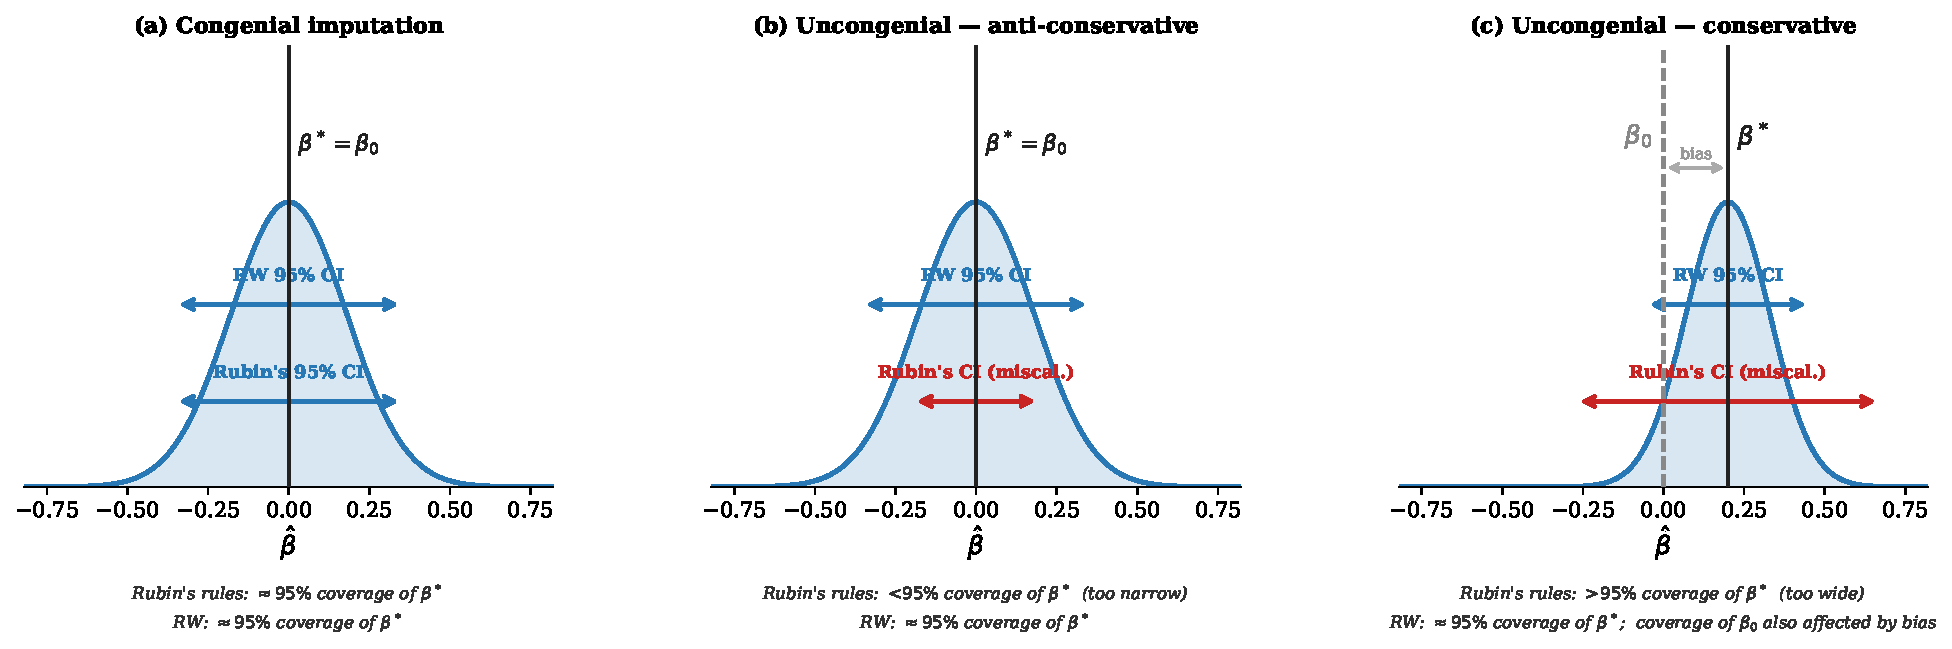
\includegraphics[width=\textwidth]{figures/toy_example.pdf}
  \caption{Conceptual illustration of variance calibration for
  multiply imputed estimators.
  Each panel shows the sampling distribution of \(\hat\beta\) (shaded
  curve) under repeated study replications, the probability limit
  \(\beta^\ast\) (solid vertical line), and, in panel~(c), the
  data-generating coefficient \(\beta_0\) (dashed vertical line).
  Horizontal brackets indicate 95\% confidence intervals from RR (lower bracket, red when miscalibrated) and from the RW
  estimator (upper bracket, blue).
  Panel~(a): congenial imputation, both intervals are correctly
  sized and achieve approximately 95\% coverage of \(\beta^\ast\).
  Panel~(b): uncongenial, anti-conservative case, the RR interval
  is too narrow, leading to under-coverage of \(\beta^\ast\); the RW
  interval is correctly sized.
  Panel~(c): uncongenial, conservative case with estimator bias
  (\(\beta^\ast\ne\beta_0\)), the RR interval is too wide,
  producing over-coverage of \(\beta^\ast\); coverage of \(\beta_0\)
  depends additionally on the bias \(\beta^\ast-\beta_0\).
  The primary simulation diagnostic in
  Section~\ref{simulation-studies} is coverage of \(\beta^\ast\),
  because it isolates variance calibration from point-estimator bias.}
  \label{fig:schematic}
\end{figure}
%======================================================================
% 2.4 Variance estimation using Robins-Wang
%======================================================================
\subsection{Variance estimation using Robins--Wang}
\label{robinswang-variance-components}
\subsubsection{The three sources of variability}
We begin by giving an overview of each component of the Robins--Wang
(RW) variance estimator, and then provide formal definitions.  The
multiply imputed estimator \(\hat\beta\) solves an averaged
complete-data estimating equation, and its repeated-sampling
variability has exactly three first-order sources.
\emph{Source 1: analysis-score variability.}  Even if the
imputation-model parameter \(\psi\) were known exactly and held fixed,
\(\hat\beta\) would still vary across repeated study replications,
because the analysis scores \(U_i(\beta)\) fluctuate with the observed
data.  This is the same variability that ordinary complete-data
sandwich inference would estimate.  It does not vanish as the number of
imputations \(m\) grows, because it reflects between-subject variation
in the analysis, not between-imputation variation.
\emph{Source 2: imputation-parameter uncertainty.}  In practice,
\(\psi\) is estimated from the observed data, and this estimation
uncertainty propagates into \(\hat\beta\) through the imputed values.
The propagation has two steps.  First, \(\hat\psi\) fluctuates around
its limit across replications, with magnitude governed by its influence
function \(d_i\) (Section~\ref{data-notation}).  Second, those
fluctuations shift the imputed values, which in turn shift the analysis
score; how strongly depends on the sensitivity of the analysis score to
the imputation score.  These quantities are defined through the
parametric imputation score; Section~\ref{extension-2} shows how a
smooth donor-selection working law supplies the analogous score for
PMM.
\emph{Source 3: cross-covariance.}  Sources 1 and 2 are not
independent, because the same observed records drive both the analysis
score and the imputation-parameter estimator.  A subject that pushes
\(\hat\psi\) in one direction also tends to shift the analysis score in
a correlated direction.  Ignoring this dependence would misrepresent
the true variance, so a cross-covariance term accounts for it
explicitly.
How does RR compare?  The within-imputation variance is an
estimate of Source 1, and the between-imputation variance is an
approximation of Source 2.  However, their additive combination is
valid only under congeniality.  When the imputation and analysis
procedures are uncongenial, the between-imputation component conflates
Sources 2 and 3 incorrectly: it inflates the variance in settings where
the imputation model uses information beyond the analysis (as in the GS
validation benchmark, where RR was conservative by \(29\%\)), and
deflates it where the analysis exploits structure the imputation model
does not capture (as in the RW missing-data benchmark, where RR is
anti-conservative).  The RW estimator builds all three sources directly
from estimating-equation quantities, which is what makes it valid
without congeniality.  The formal definitions below make these three
sources precise.
\subsubsection{Components of the RW variance estimator}
We first present the RW variance estimator in the setting RW originally
considered, in which all missing values are drawn from a parametric
imputation model indexed by \(\psi\); in
Section~\ref{improved-variance} we extend the RW variance estimator to
chained-equation and PMM imputation.  Beyond the influence function
\(d_i\) of \(\hat\psi\) introduced in Section~\ref{data-notation}, one
further score-type object enters the RW calculation: the missing-value
score \(S_{\mathrm{mis},i}\), the imputation-model score evaluated at
the imputed value for record \(i\).  In sample form the influence
function is
\[
d_i
=
-\Bigl\{P_n\,\partial S_{\mathrm{obs},i}/\partial\psi^\top\Bigr\}^{-1}
S_{\mathrm{obs},i}.
\]
Because \(S_{\mathrm{obs},i}\) is zero for records with nothing observed
for the imputed variable, \(d_i\) is supported only on records that
contribute to the imputation fit, and the sums defining \(\widehat\alpha\)
and \(\widehat C\) below run effectively over those records.
\citet{robins2000inference} express the first-order variance of
\(\hat\beta\) using \(U\), \(S_{\mathrm{mis}}\), and \(d\).  In sample
form, the sandwich variance estimator is
\[
\widehat\Gamma
=
\frac{1}{n}\widehat\tau^{-1}\widehat\Delta\,\bigl(\widehat\tau^{-1}\bigr)^{\!\top},
\qquad
\widehat\Delta
=
\widehat\Omega
+\widehat\kappa\widehat\alpha\widehat\kappa^\top
+\widehat C .
\]
The three matrices inside \(\widehat\Delta\) are empirical second moments
of order one; the leading \(1/n\) converts the sandwich limit for
\(\sqrt n(\hat\beta-\beta^\ast)\) into the finite-sample variance of
\(\hat\beta\).  We keep this scaling explicit so that \(\widehat\Delta\)
is directly comparable with the population formulas in
\citet{robins2000inference}.
The \emph{bread} \(\widehat\tau\) is the average derivative of the
completed-data estimating equation with respect to \(\beta\),
\[
\widehat\tau
=
\frac{1}{nm}\sum_{p=1}^m\sum_{i=1}^n
\left.\frac{\partial U_i^{(p)}(\beta)}{\partial\beta^\top}
\right|_{\beta=\hat\beta}.
\]
It linearises the estimating equation around the solution
\(\hat\beta\), converting the sandwich into units of
\(\mathrm{Var}(\hat\beta)\).  We use \emph{bread} and \emph{meat} in
their standard sandwich-variance sense: \(\widehat\tau\) estimates the
expected derivative of the averaged estimating function, and
\(\widehat\Delta\) estimates the variance of its subject-level
contributions.
As described above, the \emph{meat} \(\widehat\Delta\) is made up of three
components, corresponding to the three sources of variance.  We now give
their explicit forms.
\medskip
\noindent\textit{Source 1: analysis-score covariance.}\enskip
The first piece is the outer product of each subject's
imputation-averaged analysis score \(\bar U_i\).  Averaging over
imputations within each subject eliminates imputation noise, leaving
only the between-subject variation in the analysis score that would
exist even if \(\psi\) were known:
\[
\widehat\Omega
=
\frac{1}{n}\sum_{i=1}^n
\bar U_i(\hat\beta)\,\bar U_i(\hat\beta)^\top.
\]
\medskip
\noindent\textit{Source 2: imputation-parameter uncertainty.}\enskip
The second piece is assembled from two building blocks.  The matrix
\(\widehat\kappa\) measures how sensitively the analysis score responds
to a change in the imputed value: it is the sample cross-moment of the
analysis score \(U_i^{(p)}\) and the missing-value score
\(S_{\mathrm{mis},i}^{(p)}\), which is the gradient of the imputation
log-likelihood with respect to \(\psi\) evaluated at the imputed value.
A large \(\widehat\kappa\) means that small shifts in \(\psi\), and hence in the imputed values, substantially move the analysis score. The matrix \(\widehat\alpha\) is the variance of the influence contribution \(d_i^{(p)}\) across subjects and imputations; it measures
how much \(\hat\psi\) fluctuates as the observed data change.  Together,
\[
\widehat\kappa
=
\frac{1}{nm}\sum_{p=1}^m\sum_{i=1}^n
U_i^{(p)}(\hat\beta)\,S_{\mathrm{mis},i}^{(p)\top},
\qquad
\widehat\alpha
=
\frac{1}{nm}\sum_{p=1}^m\sum_{i=1}^n
d_i^{(p)}d_i^{(p)\top},
\]
and the contribution of imputation-parameter estimation uncertainty to
\(\mathrm{Var}(\hat\beta)\) is \(\widehat\kappa\widehat\alpha\widehat\kappa^\top\).
\medskip
\noindent\textit{Source 3: cross-covariance.}\enskip
The third piece corrects for the dependence between Sources 1 and 2.
Because subject \(i\) simultaneously contributes to \(\bar U_i\) (the
analysis score) and to \(\bar d_i\) (the influence on \(\hat\psi\)),
the two sources are correlated at the individual level.  Writing
\(\bar d_i = m^{-1}\sum_{p=1}^m d_i^{(p)}\) for the
imputation-averaged influence contribution, the cross-covariance is
\[
\widehat C
=
\frac{1}{n}
\Bigl[
\widehat\kappa
\Bigl\{\sum_{i=1}^n \bar d_i\,\bar U_i^\top\Bigr\}
+
\Bigl\{\sum_{i=1}^n \bar U_i\,\bar d_i^\top\Bigr\}
\widehat\kappa^\top
\Bigr]
=
\frac{1}{n}
\bigl[
\widehat\kappa\,\bar d^\top \bar U
+
\bar U^\top\bar d\,\widehat\kappa^\top
\bigr],
\]
where \(\bar U\) and \(\bar d\) are the \(n\times q\) and \(n\times c\)
matrices with rows \(\bar U_i^\top\) and \(\bar d_i^\top\), and
\(c=\dim(\psi)\) as introduced in Section~\ref{data-notation}.  The
symmetrisation (adding the transpose) ensures \(\widehat\Delta\) is
symmetric.  The RR variance estimator implicitly sets a version of this
term to zero, which is one reason it is miscalibrated under
uncongeniality.